\chapter{Нейросетевые методы машинного обучения для задач обработки естественного языка}\label{ch:nn} 
 
\section{Основные понятия}
\subsection{Определение нейросетевых методов машинного обучения}
Нейросетевые методы машинного обучения - это методы, основанные на использовании искусственных нейронных сетей. В данной работе рассматривается класс искусственных нейронных сетей, представляющих собой совокупность слоев с функциями активации, таких, что подаваемые на вход данные проходят через различные слои по очереди, где каждый слой представляет собой многомерную функцию многих переменных. Итоговый выход нейронной сети подается в функцию потерь, после чего функция потерь оптимизируется методом обратного распространения ошибки. 
\subsection{Метод обратного распространения ошибки}
Метод обратного распространения ошибки - один из методов «обучения с учителем», то есть подход, при котором модель учится решать задачу, чтобы соответствовать набору примеров входных/выходных данных. Для определения того, насколько ответ, данный нейронной сетью, соответствует требуемому, вводится функция потерь. Далее выполняется поиск точки минимума функции потерь в пространстве параметров искусственной нейронной сети для данного набора примеров входных данных. Параметры искусственной нейронной сети включают в себя синаптические веса и сдвиги нейронов. Впервые данный метод был предложен в 1974 году~\cite{werbos_1974}. Чтобы данный метод работал, функция потерь и все слои нейронной сети должны иметь ненулевые частные производные по параметрам ИНС на достаточно большой части своих областей определения.
Данный метод оказался очень эффективным, так как он применим к сетям с практически любыми архитектурами. С использованием этого метода связано возрождение интереса к исследованию области нейронных сетей, которая в восьмидесятых годах называлась «коннекционизмом». 

Все самые главные достижения в области нейронных сетей в 21 веке были связаны именно с применением нейросетевых подходов. Хотя существовали и достижения на основе иных подходов, как например, условные случайные поля~\cite{lafferty_2004}, метрика BLEU (пословная схожесть перевода с оригиналом)~\cite{papineni_2001}, латентное разложение Дирихле~\cite{blei_2003}, автоматическая генерация данных из имеющейся базы знаний~\cite{mintz_2009}, главную роль играли именно нейросетевые подходы. Ниже будут кратко описаны основные шаги в их развитии.

\subsection{Полносвязные нейронные сети}
Одним из классических видов нейронных сетей являются полносвязные нейронные сети - сети, состоящие из полносвязных слоев. Будем называть полносвязным слоем с M нейронами взвешенную сумму значений входного вектора x размерности N, к каждому элементу которой затем применяется функция активации $\sigma(y)$:

\begin{equation}
\begin{split} 
\color{black}z=\sigma(y)\\
\color{black}y=W_{0}+W_{1}X
\end{split}
\label{nn:0}
\end{equation}
где $W_{1}$ - матрица весов (weights) полносвязного слоя размерности $N*M$, $W_{0}$ - матрица биасов (bias) полносвязного слоя размерности M, $\sigma$ - некая нелинейная функция активации.

В качестве функции активации обычно используется softmax:

\begin{equation}
  \sigma(z_i) = \frac{e^{z_{i}}}{\sum_{j=1}^K e^{z_{j}}} \ \ \ for\ i=1,2,\dots,K
\label{softmax}
\end{equation}

или relu:
\begin{equation}
  relu(z_i) = max(0, z_i)
\label{relu}
\end{equation}

где $i$ - индекс $K$-мерного вектора $z$.

Для регуляризации в таких слоях (как и в других, более сложных) применяется также дропаут, предложенный в~\cite{dropout}. При использовании данного метода некий процент элементов выходного вектора (как правило, 10-20\%) приравнивается к нулю. Такая техника мешает «переобучению» нейронной сети, улучшая тем самым ее обобщающую способность.

\subsection{Токенизация}

Перед обработкой естественного текста этот текст токенизируется, или разбивается на элементарные единицы - токены. Один токен соответствует одному слову либо же одной более мелкой его единице(букве или слогу) в зависимости от метода токенизации. Для нижеописанного метода Word2Vec токеном является 1 слово, для нижеописанной архитектуры BERT - слово либо слог.

\subsection{Нейросетевые языковые модели}

Языковое моделирование - это задача предсказания следующего слова в тексте с использованием предыдущих. У языкового моделирования есть простейшие практические приложения - умная клавиатура и пр. Первые подходы к языковому моделированию основывались на марковских моделях\cite{kneser_1995} . Позднее, в 2003 году, была предложена первая нейросетевая языковая модель \cite{bengio_2003}, изображенная на рисунке \ref{fig:Neuro1-Feedforward}. 
Модель берет из таблицы C векторные представления N предыдущих слов, потом эти представления соединяются и подаются в скрытый слой, оттуда - в функцию активации softmax. В дальнейшем вместо данных сетей стали применяться рекуррентные сети \cite{mikolov_2010} или сети с долгосрочной памятью \cite{hochreiter_1997}.%todo - firmula here
Языковое моделирование является частью таких более поздних продвижений в области обработке текста, как векторные представления слов, предварительно обученные языковые модели, модели seq2seq и т.д.

\begin{figure}[ht]
 \centerfloat{
  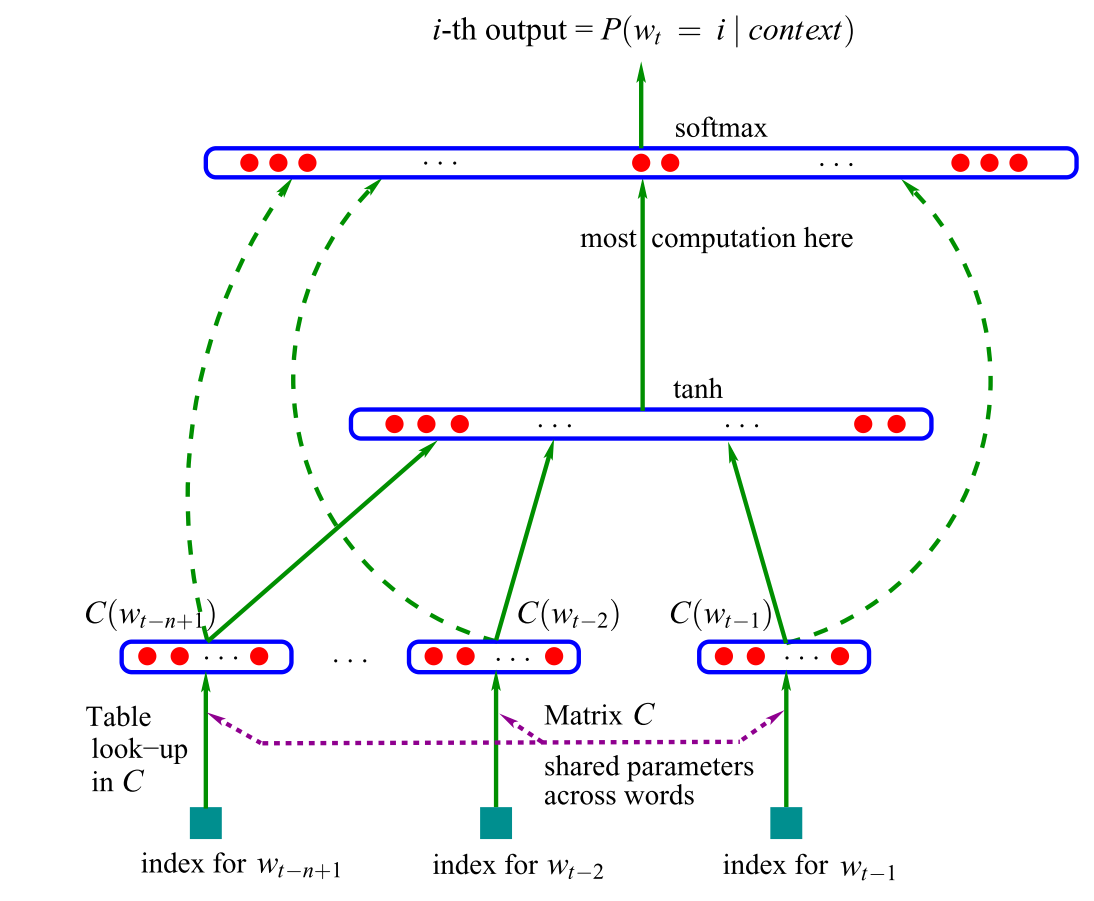
\includegraphics[width=\textwidth]{images/Neuro1-Feedforward_.png}
 }
 \caption{Первая нейросетевая языковая модель}\label{fig:Neuro1-Feedforward}
\end{figure}


\subsection{Векторные представления слов}
Разреженные представления слов в обработке естественного текста использовались достаточно давно. Хотя первая нейросетевая языковая модель была предложена еще в 2003 году~\cite{bengio_2003}, основное нововведение~\cite{mikolov_2013}, предложенное в 2013 году - архитектура Word2vec - позволило гораздо успешнее обучать векторные представления слов(т.е проводить их векторизацию). Word2vec существует в двух вариантах - CBOW и skip-gram, которые подробнее представлены на рисунке \ref{fig:Neuro2-Word2Vec}. Они различаются по своей цели: один предсказывает центральное слово на основе окружающих слов, а другой делает обратное.


\begin{figure}[ht]
 \centerfloat{
  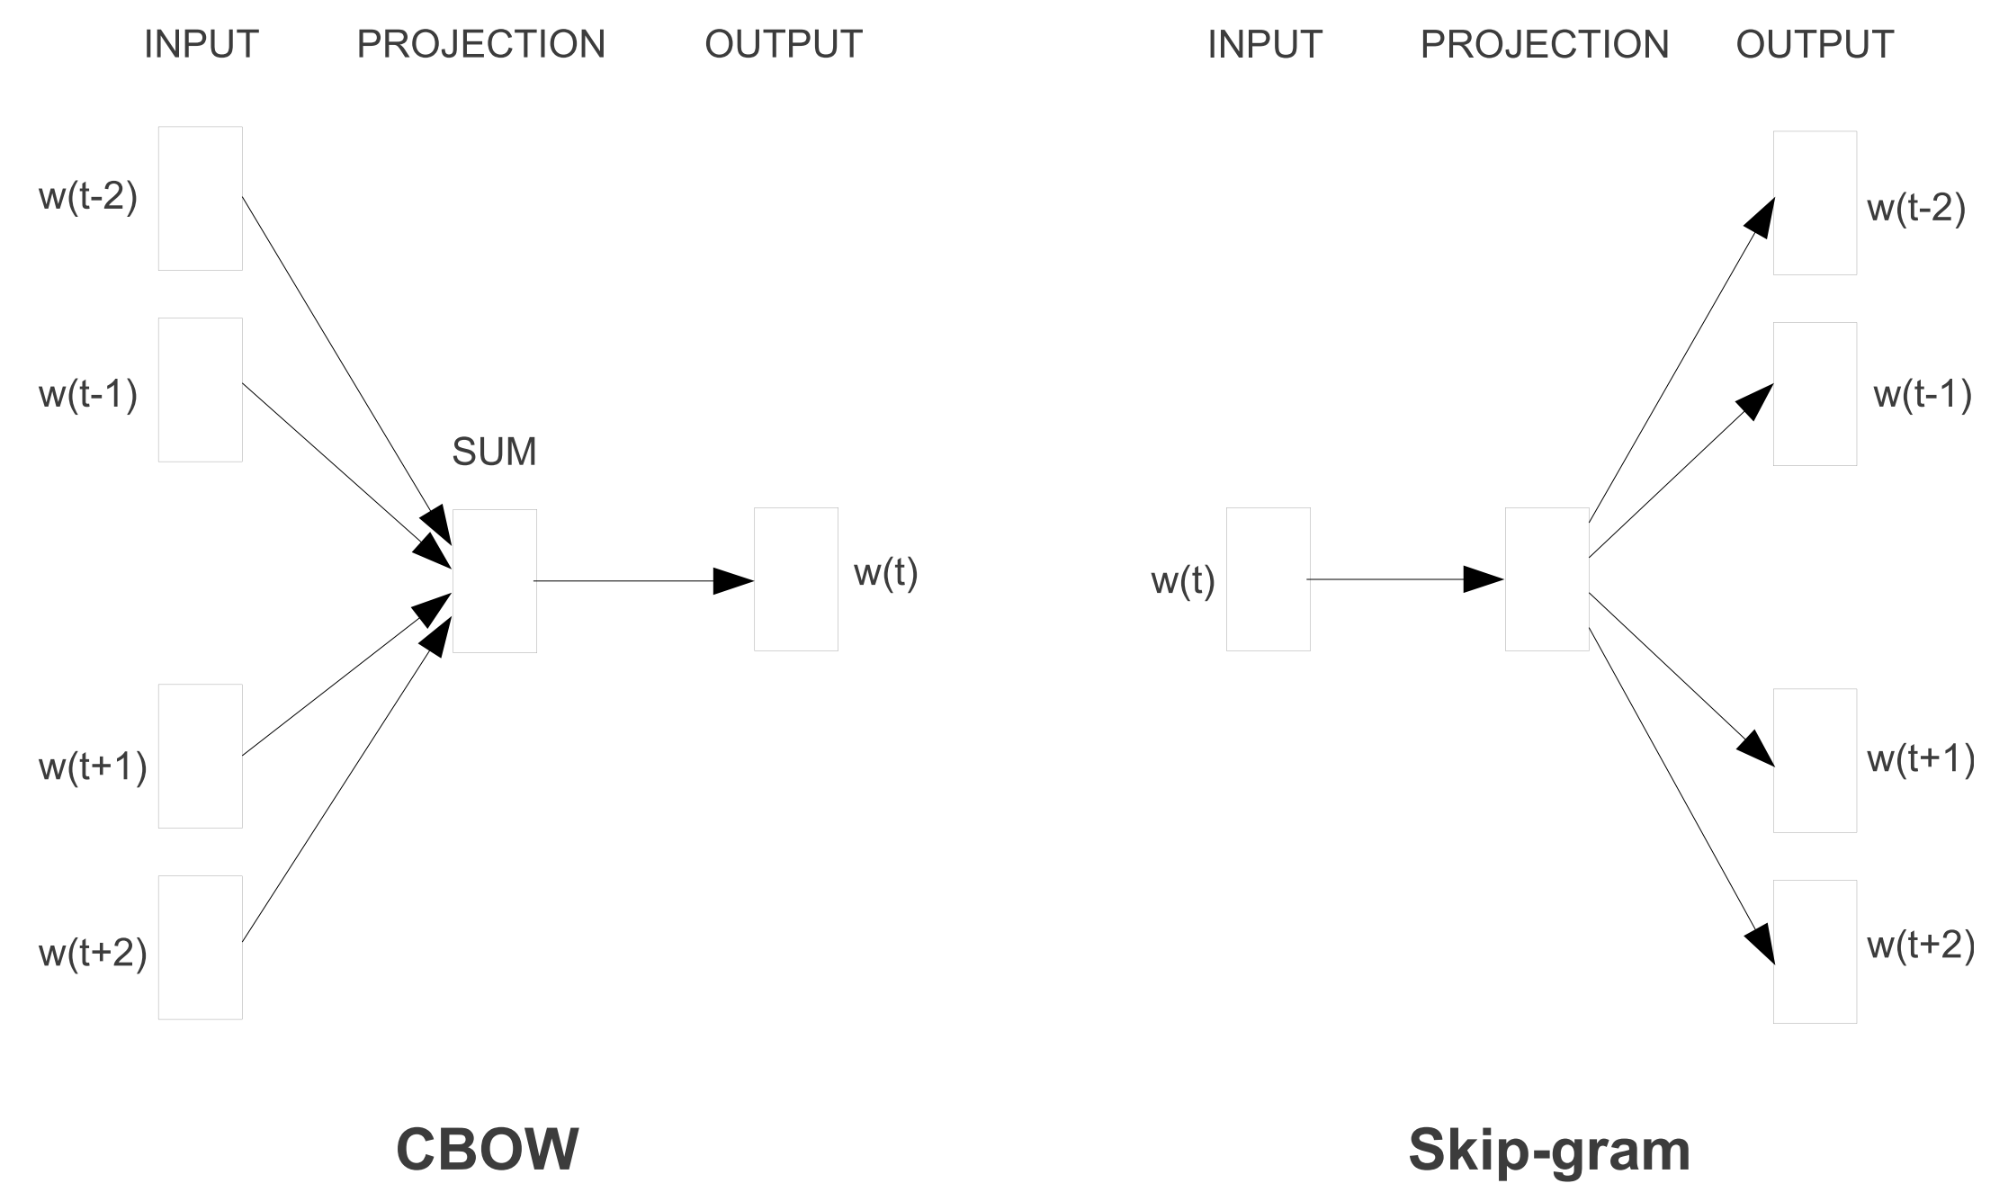
\includegraphics[width=\textwidth]{images/Neuro2-Word2Vec_.png}
 }
 \caption{Word2Vec}\label{fig:Neuro2-Word2Vec}
\end{figure}

Использование модели для большого обучающего корпуса позволяет модели выучить такие понятия, как пол, время глагола, или отношения типа страна-столица. 

%\iffalse
\subsection{Нейронные сети для обработки текста}
В 2013-2014 годах нейросети (в первую очередь - рекуррентные, сверточные и рекурсивные) стали активно использоваться для обработки текста.  Наиболее широко в то время использовались три основных типа нейронных сетей: рекуррентные нейронные сети, сверточные нейронные сети и рекурсивные нейронные сети. Они будут подробнее описаны ниже, в разделах \ref{ch:nn:rnn}, \ref{ch:nn:cnn} и \ref{ch:nn:rcnn}.

\subsubsection{Рекуррентные нейронные сети}\label{ch:nn:rnn}
Рекуррентные нейронные сети (RNN) лучше всего подходят для работы с динамическими входными последовательностями, из которых и состоит естественный язык.  Первые рекурсивные сети были предложены Элманом в 1990 году~\cite{elman_1990}, но в 1997 году на их место пришли предложенные Шмитхубером сети долговременной памяти(LSTM) \cite{hochreiter_1997}, которые оказались более устойчивыми к проблеме исчезания/взрыва градиентов. В 2013 году Илья Суцкевер предложил в своей диссертации новый, более эффективный метод обучения LSTM \cite{suskever_2013}. Также в 2013 году Грэйвсом были предложены двунаправленные LSTM~\cite{graves_2013}, которые обычно используется для работы с левым и правым контекстом. Визуализацию ячейки LSTM можно увидеть на рисунке \ref{fig:Neuro3-LSTM}.  


\begin{figure}[ht]
  \centerfloat{
    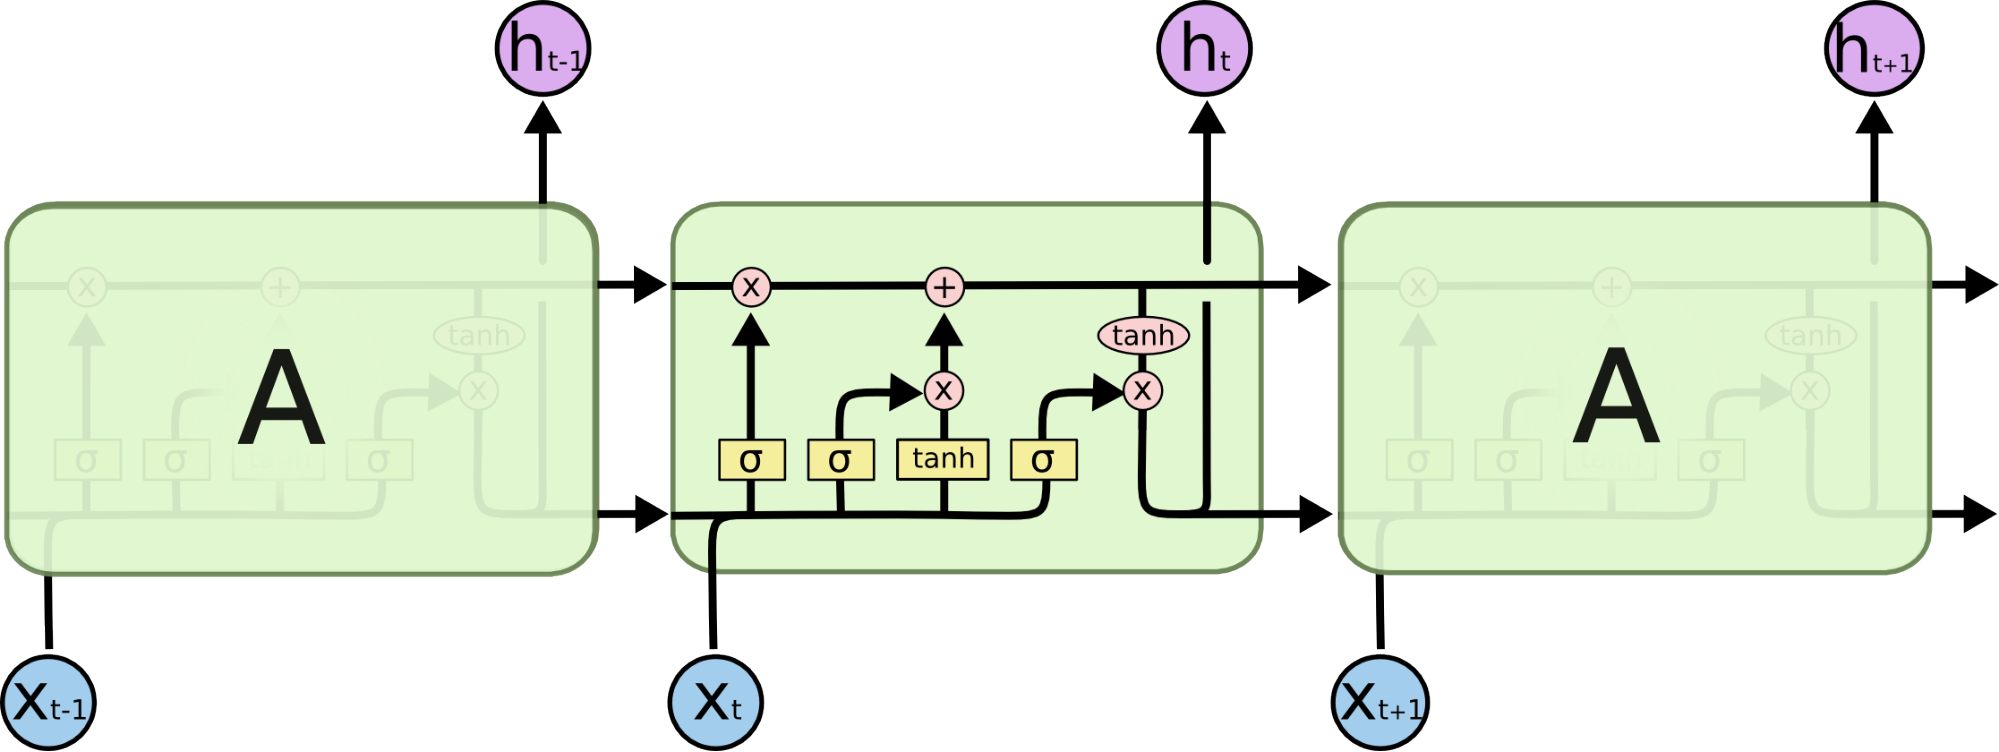
\includegraphics[width=\textwidth]{images/Neuro3-LSTM_.png}
  }
  \caption{Визуализация ячейки LSTM}\label{fig:Neuro3-LSTM}
\end{figure}


\subsubsection{Сверточные нейронные сети}\label{ch:nn:cnn}
Сверточные нейронные сети работают на основе операции свертки в двух измерениях, в 2014 году \cite{kalchbrenner_2014} они начали применяться в области обработки естественного языка. Преимуществом сверточных нейронных сетей, по сравнению с рекуррентными, является их распараллеливаемость. На рисунке \ref{fig:Neuro4-CNN} показан пример сверточной нейронной сети, используемой в обработке текста.


\begin{figure}[ht]
  \centerfloat{
    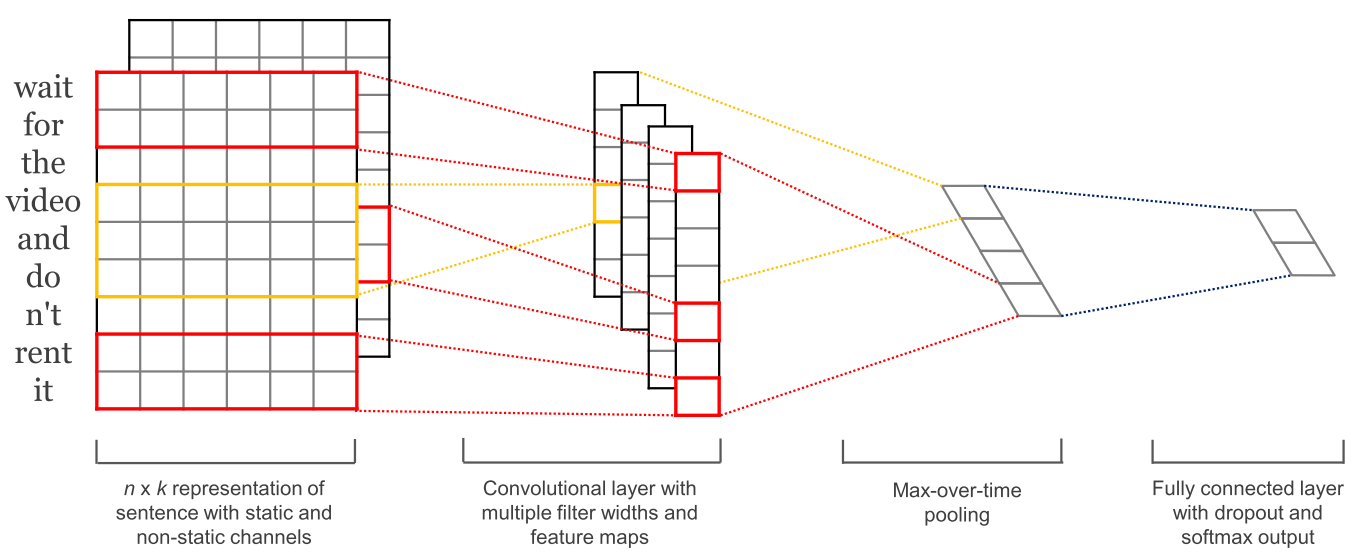
\includegraphics[width=\textwidth]{images/Neuro4-CNN_.png}
  }
  \caption{Пример сверточной нейронной сети}\label{fig:Neuro4-CNN}
\end{figure}

\subsubsection{Рекурсивные нейронные сети}\label{ch:nn:rcnn}
Хотя рекуррентные и сверточные нейросети рассматривают естественный язык как последовательность, по своей сути он иерархичен: слова состоят из фраз и предложений более высокого порядка, которые сами могут быть рекурсивно объединены в соответствии с набором строго определенных правил. Это приводит к идее трактовать предложения как деревья, а не как последовательности. Воплощением данной идеи являются рекурсивные нейронные сети~\cite{socher_2013}. В отличие от рекуррентных сетей, обрабатывающих предложение слева направо или справа налево, рекурсивные сети представляют последовательность снизу вверх или сверху вниз. Новое представление в каждом узле находится при помощи составления представлений дочерних узлов. Пример рекурсивной нейронной сети изображен на рисунке \ref{fig:Neuro5-RNN}.



\begin{figure}[ht]
  \centerfloat{
    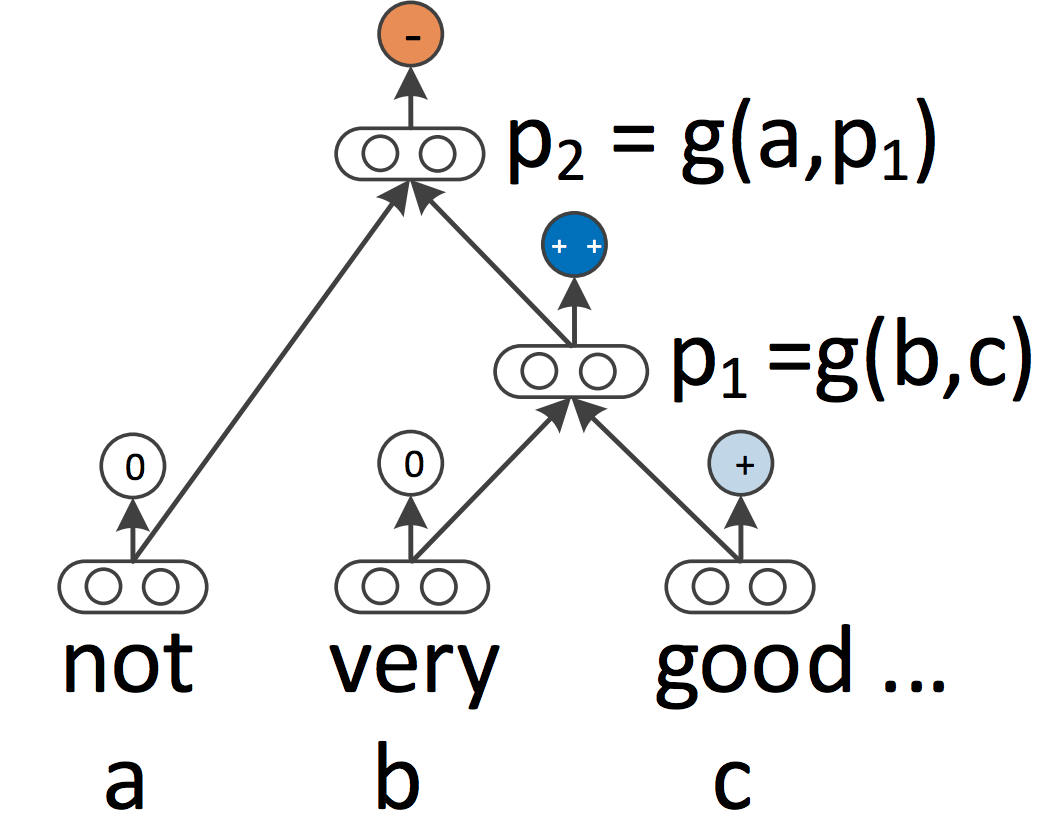
\includegraphics[width=\textwidth]{images/Neuro5-RNN_.png}
  }
  \caption{Пример рекурсивной нейронной сети}\label{fig:Neuro5-RNN}
\end{figure}
\subsection{Нейросети, основанные на памяти}
В середине 2010-х годов стали активно появляться архитектуры нейросетевых моделей, использующие память - скрытые состояния модели, при этом модель сама выбирает, что необходимо извлечь из памяти. 

Из моделей, использующих память, можно выделить сквозные сети памяти \cite{sukhbaatar_2015}, модели с динамической памятью \cite{kumar_2016}, дифференцируемые нейрокомпьютеры \cite{graves_2016}, модели с памятью «ключ-значение» \cite{miller_2016} и пр.
 
Доступ к памяти в таких моделях осуществляется при помощи «схожести» по текущему расстоянию по той или иной метрике, подобным вниманию, и память в модели обычно может записываться и считываться.  Модели отличаются тем, как они реализуют и используют память. Например, сквозные сети памяти обрабатывают ввод несколько раз и только затем обновляют память, чтобы сделать возможным несколько этапов вывода.  Нейронные машины Тьюринга имеют адресацию на основе местоположения, что позволяет им изучать простые компьютерные программы, такие как сортировка.  Модели на основе памяти, как правило, применяются к задачам, где информацию нужно хранить достаточно долго, например, моделирование языка или понимание текста. 
\subsection{Модели «предложение-в-предложение»}
В 2014 году была предложена методика обучения моделей «предложение-в-предложение» \cite{sutskever_2014} - нейросетевых моделей для отображения одной последовательности в другую. Данные модели состоят кодировщика и декодировщика. 

После токенизации предложения кодировщик обрабатывает каждый токен предложения по очереди и сжимает их в вектора скрытых состояний; на основе этих векторов скрытых состояний декодировщик шаг за шагом прогнозирует символ энкодера, который предполагается на выходе. Пример работы данной сети изображен на рисунке \ref{fig:Neuro6-Seq2Seq}.

\begin{figure}[ht]
 \centerfloat{
  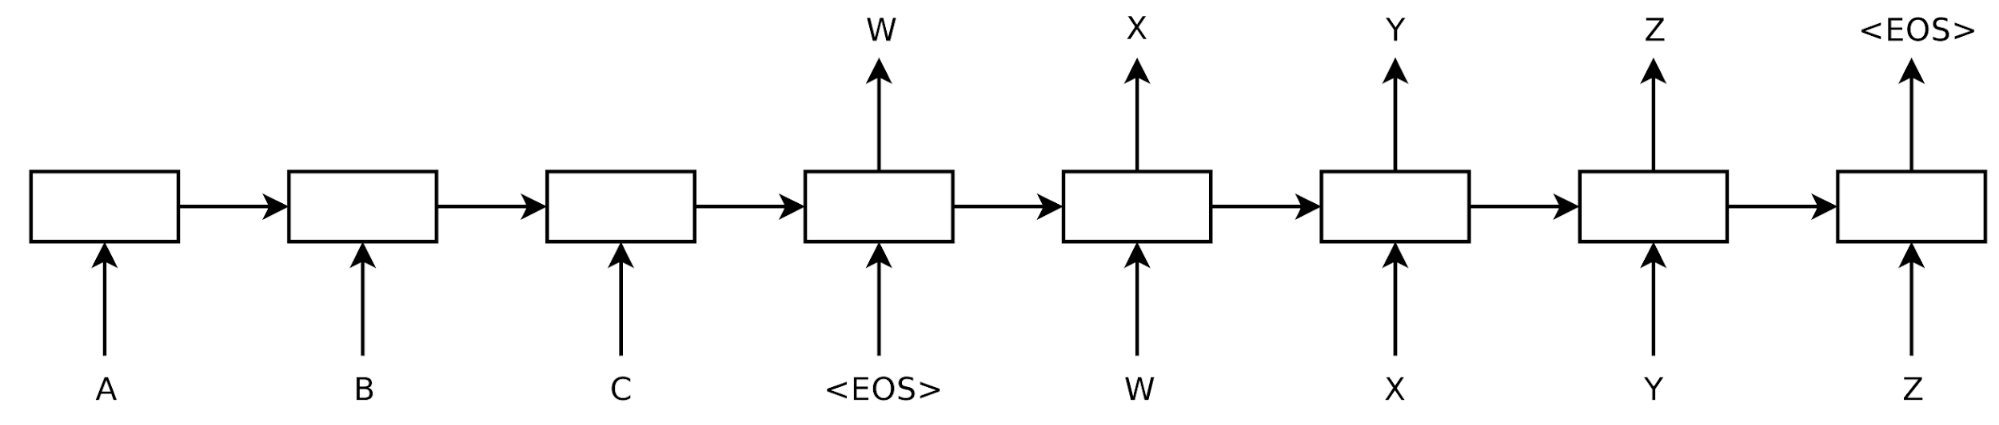
\includegraphics[width=\textwidth]{images/Neuro6-Seq2Seq_.png}
 }
 \caption{Пример сети на основе модели Seq2Seq}\label{fig:Neuro6-Seq2Seq}
\end{figure}

В 2016 году Google начал заменять свои модели машинного перевода на модели «предложение-в-предложение».\footnote{\url{https://blog.google/products/translate/found-translation-more-accurate-fluent-sentences-google-translate/}} Модели «предложение-в-предложение» могут широко применяться в любых задачах, где данные имеют конкретную структуру.
  
Кодировщик и декодировщик могут быть основаны на разных типах нейросетевых архитектур, включая архитектуру Трансформер. В следующем разделе эта архитектура рассмотрена более детально.

\section{Архитектура Трансформер и модель BERT}\label{ch:tr}

\subsection{Архитектура Трансформер}

В разделе~\ref{ch:nn} были изложены предшествовавшие этапы развития нейросетевых моделей. Но на момент проведения описываемых в данной диссертационной работе научных исследований, ключевую роль в обработке текста уже играли модели на базе архитектуры Трансформер. В связи с этим в данном разделе подробно описана данная нейросетевая архитектура. В следующем разделе \ref{ch:mtl} описаны многозадачные нейросетевые модели на основе данной архитектуры, являющиеся предметом данной диссертационной работы. 

Архитектура Трансформер была разработана в 2017 году~\cite{vaswani_2017}. Составляющие данной архитектуры - это полносвязные слои и механизм внимания(Attention). Механизм внимания был предложен авторами статьи, чтобы лучше передавать информацию из энкодера декодеру в seq2seq моделях: состояние декодировщика обновляется на основе информации от кодировщика. 

%\textbf{Self-attention} (самовнимание) - это механизм внимания, примененный к самой же входной последовательности для ее обновления, Данное понятие было предложено в работе~\cite{lin_2017}. Там оно применялось для векторизации предложения, что было необходимо для решения задач классификации текста. В архитектуре Трансформер модуль Attention используется как Self-attention. 

Механизм внимания работает на основе трех матриц: Q (Query, запрос), K(Key, ключ), V(Value, значение). 

Получая на вход последовательность токенов длины $N_{queries}$, модель до применения Attention векторизует каждый из данных токенов, ставя каждому токену в соответствие вектор длины $D$. Получив тем самым представление для каждого предложения - Query размерности $N_{queries}*D$, механизм также использует Key той же размерности $N_{keys}*D$ ($N_{keys}= N_{queries})$ и Value размерности $N_{keys}*D_{v}$ для формирования взвешенного скалярного произведения в соответствии со следующей формулой:

\begin{equation}
\color{black} Attention(Q, K, V) = softmax(QK^{T}V)/sqrt(D)
\label{eq:ref}
\end{equation}

%Механизм внимания подробнее проиллюстрирован на рисунке \ref{fig:Transformer1-Attention}
%\begin{figure}[ht]
% \centerfloat{
%  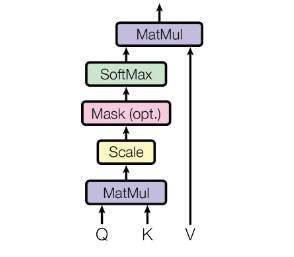
\includegraphics[width=\textwidth]{images/Transformer1-Attention_.png}
% }
% \caption{Механизм Attention.}\label{fig:Transformer1-Attention}
%\end{figure}


Внимание делится на $\sqrt{D}$, чтобы избежать затухания градиентов, подробнее описанного в \cite{hochreiter_1998}. 
Механизм внимания может широко применяться в задачах, которые требуют использования части входных данных - парсинг синтаксических зависимостей, понимание текста и пр. Механизм внимания особенно примечателен своей интерпретируемостью, так как он помогает понять, на какие части текста смотрит модель, за счет своих весовых коэффициентов.


Чтобы увеличить число вариаций, которыми представляются поступающие на вход токены, данный модуль в архитектуре Трансформер применяется h раз параллельно после чего результаты этих применений конкатенируются. При этом к матрицам Key, Value и Query предварительно применяются линейные преобразования. Иными словами:
\begin{equation}
\color{black} MultiHeadAttention(Q, K, V) = Concat(head_{1},... head_{h})W^{O} \label{tr:0}
\end{equation}
где
\begin{equation}
\color{black} head_{i} = Attention(QW_{i}^{Q},KW_{i}^{K},VW_{i}^{V}) \label{tr:1}
\end{equation},
где $W_{i}^{Q}$ - матрица линейного преобразования для запросов, имеющая размерность $D*D$, $W_{i}^{K}$ - матрица линейного преобразования для ключей, имеющая размерность $D*D$, $W_{i}^{V}$ - матрица линейного преобразования для значений, имеющая размерность $D*D_{v}$



Подобное применение self-attention называется «Multi-head self-attention» (многоголовое самовнимание). Оно проиллюстрировано на рисунке \ref{fig:Transformer2-MultiHeadSelfAttention}.



\begin{figure}[ht]
 \centerfloat{
  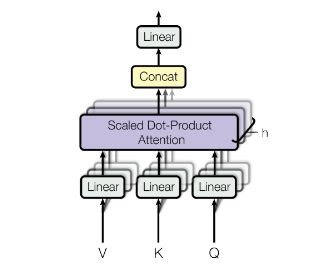
\includegraphics[width=\textwidth]{images/Transformer2-MultiHeadSelfAttention_.png}
 }
 \caption{Многоголовое самовнимание.}\label{fig:Transformer2-MultiHeadSelfAttention}
\end{figure}


Число голов h выбирается авторами модели вручную. Как правило, чем больше слоев у модели Трансформер, тем больше голов. 
В архитектуре Трансформер механизм внимания используется, чтобы передавать информацию с предыдущего слоя на следующий. Механизм внимания применяется к самой входной последовательности.


В архитектуру Трансформер входят повторяющиеся полносвязные слои и механизмы внимания. Они образуют Трансформер слои, из которых состоят кодировщик и декодировщик. Кодировщик состоит из некого числа N повторящихся слоев типа «многоголовое самовнимание + полносвязный слой», где полносвязный слой применяется к каждому элементу последовательности независимо. В кодировщике также используются остаточные (residual) связи вокруг этих слоев, описанные в \cite{he_2016}, и нормализации слоя, описанная в \cite{ba_2016}.

Декодировщик состоит из N повторяющихся слоев типа «многоголовое самовнимание + внимание на последний слой кодировщика + полносвязный слой». 
 Подробнее модули кодировщика и декодировщика изображены на рисунке \ref{fig:Transformer4-EncoderDecoder}. 

\begin{figure}[ht]
 \centerfloat{
  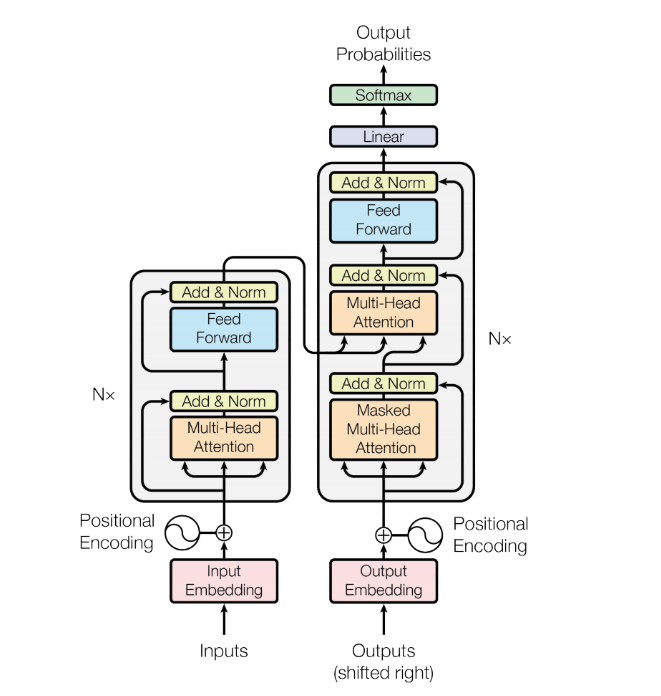
\includegraphics[width=\textwidth]{images/Transformer4-EncoderDecoder_.png}
 }
 \caption{Модули кодировщика и декодировщика в архитектуре Трансформер.}\label{fig:Transformer4-EncoderDecoder}
\end{figure}

При этом при применении многоголового самовнимания в кодировщике
\begin{equation}
  Q = K = V = X_e
\end{equation},
где X\_e - векторные представления токенов предложения, которые поступают в кодировщик.
При применении многоголового самовнимания в декодировщике
\begin{equation}
  Q = K = V = X_d
\end{equation},
где X\_d - векторные представления токенов предложения, которые поступают в декодировщик.
При применении внимания на последний слой кодировщика
\begin{equation}
  Q = K = X_e
\end{equation}
\begin{equation}
  V = X_d
\end{equation}
%https://alibaba-cloud.medium.com/self-attention-mechanisms-in-natural-language-processing-9f28315ff905

 Заметим, что, поскольку декодировщик предсказывает следующее слово по предыдущим, он не может видеть информацию о будущих словах во время обучения. Поэтому в декодировщике используется маскированное само-внимание(masked self-attention). Модуль MASK «маскирует» следующие слова.
Заметим, что порядок элементов входной последовательности в оригинальной архитектуре Трансформер никак не используется, так как каждая из операций в Трансформер слое, что в кодировщике, что в декодировщике, происходит независимо для разных элементов последовательности. 

В статьях \cite{devlin_2018,gehring_2017,vaswani_2017} предложен следующий способ добавления информации о положении данного токена во входной последовательности - векторные представления позиций (position embeddings). Данные векторные представления суммируются со входными векторными представлениями. Они могут задаваться аналитически, а могут обучаться вместе с параметрами всей модели.
Архитектура Трансформер получила большое развитие за последние годы. Так, в репозитории компании HuggingFace \cite{na_website_ndaa} находится более 16 тысяч моделей, имеющих данную архитектуру, в том числе дообученных на конкретную задачу. 

Самой популярной моделью на основе архитектуры Трансформер является модель BERT, которая широко использовалась в дальнейшей работе. Эта модель описана подробнее в следующем подразделе. 

\subsection{Модель BERT}

BERT (Bidirectional Encoder Representations from Transformer)~\cite{devlin_2018} - основанные на архитектуре Tрансформер модели для обработки естественного текста, предобученные одноимённым методом на задачах предсказания токена по контексту и определения того, могут ли данные 2 предложения следовать одно за другим. 

BERT - это универсальная архитектура. На базе BERT могут работать различные модели NLP - модели классификации одного предложения, классификации пары предложений, регрессии, выбора из вариантов, вопросно-ответные и так далее. Модели на основе BERT значительно превзошли модели предыдущего поколения для обработки естественного языка. 
Данный метод имеет следующие ключевые особенности:
\begin{itemize}
\item[*] Модель BERT состоит только из слоев-кодировщиков, без слоев-декодировщиков. Каждый слой-кодировщик работает с выбором предыщушего слоя.
\item[*] BERT обрабатывает всю последовательность одновременно. По определению авторов, это двунаправленная (bidirectional) обработка. Отличие данного способа обработки от применяемого в двунаправленных рекуррентных сетях заключается в следующем: в двунаправленных сетях обработка входных данных производится по одному токену слева направо и справа налево, последовательно. А в нейронных сетях, имеющих архитектуру Трансформер, включая BERT, обработка каждого токена производится параллельно, при этом каждый токен имеет доступ при помощи механизма внимания ко всем остальным токенам. 
\item[*] BERT предобучается без учителя, или точнее, с самообучением (self supervised learning). Предобучение модели BERT требует большого объёма неразмеченных текстов, разметку для которых при этом можно получить из самих этих текстов, используя уже имеющуюся в них информацию.
\end{itemize}
Обучение модели BERT делится на 2 стадии: предобучение(pretraining) на большом объеме неразмеченных текстов и дообучение(finetuning) на относительно небольшом объёме данных, специфических для каждой конкретной задачи. 

Предобучение производится на две задачи. Первой из двух задач является Маскированное языковое моделирование (Masked Language Modeling, MLM). В данной задаче некоторые входящие токены последовательности маскируются, заменяясь на служебный токен [MASK]. Модель BERT учится предсказывать маскированные токены. Так как токен [MASK] не используется при дообучении (fine-tuning) модели, то замена производится следующим образом: каждый из 15\% случайно выбранных токенов с вероятностью 80\% заменяется на токен [MASK] (I feel very well заменяется, например, на I feel [MASK] well), с вероятностью 10\% заменяется на другой токен (I feel very well - >I feel blue well), с вероятностью 10\% не изменяется (I feel very well - >I feel very well). Эти 15\% токенов предсказываются на основе векторных представлений на финальном слое модели BERT. В качестве функции потерь используется кросс-энтропия, в качестве финальной функции активации Softmax. 

Помимо описанной выше задачи, модель BERT также необходимо научить работать с текстом не только на уровне одного предложения, но и на уровне нескольких предложений. Для этого модель BERT также учится предсказывать, может ли одно предложение встретиться после другого или нет. Данная задача называется Next Sentence Prediction (NSP). В качестве положительных примеров в набор данных добавляются пары предложений, встретившиеся в обучающей выборке и стоявшие рядом друг с другом. В качестве отрицательных примеров - случайные пары предложений. Два предложения разделяются служебным токеном [SEP] , перед ними ставится другой служебный токен [CLS], а после всех токенов - служебный токен [EOS].Пример представления: «[CLS] I wake up [SEP] I go to work [EOS]» для предложений «I wake up» и «I go to work». Финальное векторное представление токена [CLS] используется линейным слоем «наверху» модели BERT для классификации этой пары предложений. Подбор пары предложений для модели BERT-BASE осуществляется таким образом, чтобы их суммарная длина не превышала 512 токенов. У 90\% пар длина не превышала 128 токенов. Функцией потерь, как и в предыдущем пункте, является кроссэнтропия, функцией активации - Softmax.

Векторные представления каждого токена из сформированной по указанным выше правилам входной последовательности токенов суммируются также ещё с 2 видами векторных представлений: это представления сегмента последовательности (обозначающие, к первому предложению или ко второму относится данный токен) и представления позиции токена в последовательности (добавляющие информацию о позиции токена). Наглядное представление можно увидеть на рисунке \ref{fig:Transformer5-BERTTokenTypes}. 

\begin{figure}[ht]
 \centerfloat{
  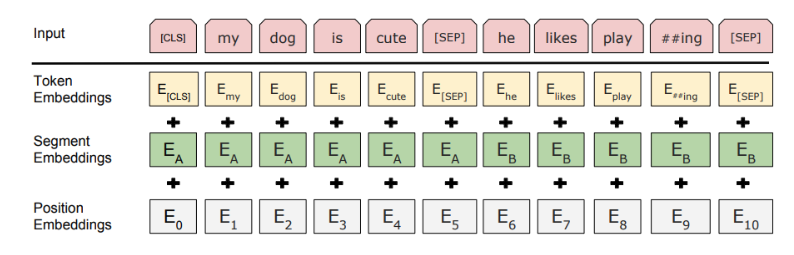
\includegraphics[width=1.0\textwidth]{images/Transformer5-BERTTokenTypes_.png}
 }
 \caption{Три типа представления токенов в модели BERT}\label{fig:Transformer5-BERTTokenTypes}
\end{figure}
Модель BERT предобучалась на 2 наборах данных. Это набор данных BooksCorpus, имеющий 800 миллионов слов~\cite{zhu_2015}, и набор данных из английской Википедии, содержащей 2.5 миллиардов слов \cite{devlin_2018}. 

Дообучение модели BERT может производиться на любых, даже небольших наборах данных. Как и при решении задачи Next Sentence Prediction, в задачах классификации и регрессии ответ модели предсказывается линейным слоем по финальному векторному представлению [CLS] токена. В оригинальной статье показаны результаты модели BERT при дообучении на задачах из набора данных GLUE; цифры из данной статьи будут также использоваться в последующих разделах. 
Две основных конфигурации модели BERT, предложенные авторами оригинальной статьи - это:
\begin{itemize}
\item[*] BERT-BASE. Размерность векторного представления токена 768, 12 последовательно повторяющихся слоев Трансформер, 12 модулей self-attention в одном блоке, 110 миллионов параметров. Для обучения использовались 4 Cloud TPU 4 дня. 
\item[*] BERT-LARGE. Размерность векторного представления токена 1024, 24 последовательно повторяющихся слоя Трансформер, 16 модулей self-attention в одном блоке, 340 миллионов параметров. Для обучения использовалось 16 Cloud TPU 4 дня. 
\end{itemize}

Универсальность архитектуры BERT обуславливает возможность применения данной нейросетевой модели для решения широкого круга задач. Так, токен [SEP] позволяет ставить границы между поступающими на вход последовательностями. Это даёт возможность решать задачи классификации пар предложений и задачи ответа на вопрос (question answering), где тоже на вход подаются пары последовательности. Токен [MLM] даёт возможность для обучения векторных представлений токенов, зависящих от контекста, что позволяет решать также задачи классификации каждого токена в последовательности (распознавание именованных сущностей, классификация каждого слова по частям речи). Токен [CLS] содержит информацию обо всей последовательности, что даёт возможность применять его для решения задач классификации текста. 

Эффективность модели BERT обусловлена переносом знаний: BERT получает знания на этапе предобучения, и применяет их на этапе дообучения для решения иных задач. Таким образом, в модели BERT происходит перенос знаний. 

На момент проведения описанных в данной работе исследований, модель BERT(с определёнными модификациями) считалась стандартом в машинном обучении. В связи с этим, именно модели такого типа считались базовыми в дальнейшей работе, и при работе над многозадачными моделями приоритет в рассмотрении отдавался именно архитектурам, основанным на модели BERT. Применявшиеся в данной работе архитектуры многозадачных моделей описаны в следующем разделе \ref{ch:mtl}.

\section{Многозадачные модели}\label{ch:mtl} 

Многозадачное обучение - это метод разделения параметров между моделями, обучающимися выполнять несколько задач. Идея многозадачного обучения была впервые предложена в 1993 году~\cite{caruana_1997}. Для нейросетевых методов обработки текста оно впервые было применено в 2008 году \cite{collobert_2008}. В их модели справочные таблицы (или матрицы вложения слов) разделены между двумя моделями, обученными различным задачам, как показано на рисунке \ref{fig:MTL1}.
Использование общих параметров дает моделям возможность обмениваться низкоуровневой информацией.


\begin{figure}[ht]
 \centerfloat{
  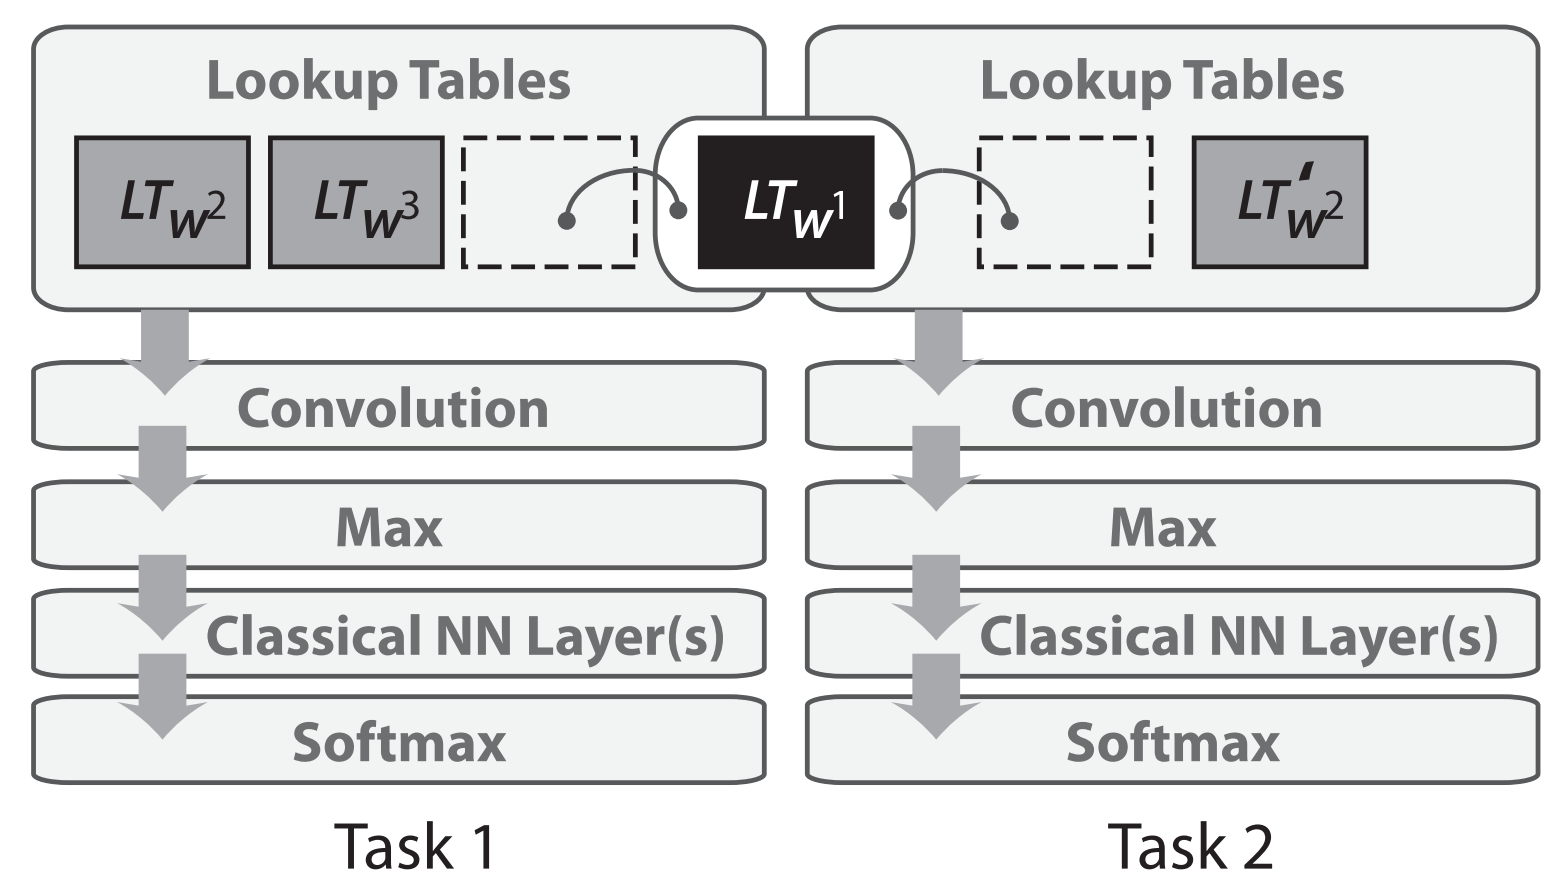
\includegraphics[width=\textwidth]{images/MTL1_.png}
 }
 \caption{Пример многозадачного обучения}\label{fig:MTL1}
\end{figure}

\subsection{Типы многозадачных архитектур}
Авторы обзора \cite{chen_2021} классифицировали архитектуры нейросетевых многозадачных моделей по следующим типам:
\begin{itemize}
\item[*] Параллельные архитектуры. Для данного типа архитектур одни и те же «общие» слои используются для примеров из каждой задачи, при этом выход «общих» слоев обрабатывается независимо своим специфическим слоем для каждой задачи. Плюсом данного типа архитектур является его достаточно высокая степень универсальности, а минусом - то, что необходимость получать одно и то же представление для каждой задачи может ограничивать адаптационные способности нейросетевой модели. К такому типу архитектур, в частности, принадлежит модель \textbf{MT-DNN}~\cite{mtdnn}, которая будет подробнее рассмотрена ниже. 
\item[*] Иерархические архитектуры. Для данного типа архитектур задачи обрабатываются зависимо друг от друга: так, результат классификации примера для одной из задач может использоваться при решении другой из задач как дополнительный входной параметр. Плюсом данного типа архитектур является возможность моделирования глубоких отношений между задачами, минусом - его негибкость. 
\item[*] Модульные архитектуры. Нейронная сеть в данных архитектурах делится на общие модули и задаче-специфичные модули, где общие модули имеют одни и те же веса для всех задач, а задаче-специфичные модули - свои веса для каждой из задач. Плюсом такого рода архитектур является возможность более точно адаптировать модель для решения нескольких задач, что даёт возможность достигать высокой степени экономии вычислительных ресурсов и хороших результатов, реализованную, в частности, в статье \cite{maziarka_2021}. Минусом же данного типа архитектур является отсутствие инвариантности по отношению к базовой модели : в отличие от параллельных архитектур, данный тип архитектур заточен под какую-то конкретную базовую нейросетевую модель, что делает замену базовой модели «под капотом» для многозадачных моделей из данного типа архитектур технически сложной. Данную архитектуру имеет, в частности, модель PAL-BERT \cite{stickland_2019}, которая будет рассмотрена в следующих разделах. 
\item[*] Генеративно-состязательные архитектуры. Для данного типа архитектур генератор и дискриминатор обучаются совместно таким образом, что дискриминатор пытается предсказать, из какой задачи пример, по его выдаваемому генератором представлению. А генератор, соответственно, пытается сгенерировать такое представление, чтобы дискриминатор мог предсказать задачу как можно хуже. Такое «состязание» генератора и дискриминатора даёт возможность генератору научиться выдавать представления примера, максимально инвариантные относительно задачи, которые в дальнейшем классифицируются скрытыми слоями на выходе, специфичными для каждой задачи. Подобный тип архитектур распространен достаточно мало в связи со своей негибкостью и нестабильностью обучения генеративно-состязательных сетей. Тем не менее, его неоспоримым преимуществом является возможность использовать большой объем неразмеченных данных для получения векторных представлений задач. 
\end{itemize}

В данной диссертационной работе исследовались возможности и особенности применения многозадачных нейросетевых моделей для обработки естественного языка. Был сделан упор на 2 нейросетевые архитектуры - модель MT-DNN \cite{mtdnn} и модель PAL-BERT \cite{stickland_2019}. Данные модели описаны подробнее в следующих разделах.

\subsection{Модель MT-DNN}\label{ch:mtl:mtdnn}
Модель MT-DNN - это многозадачная нейросетевая модель,которая относится к классу параллельных архитектурах. Данная модель, применяя один BERT к поступающему входу(с линейным pooling-слоем в конце), формирует на его базе свой собственный классификатор для каждой из задач. Модель делит все поступающие задачи на разные типы, включающие в себя, в частности:
\begin{itemize}
\item[*] Классификация текста. Пример - задачи CoLA, SST-2 из набора задач GLUE \cite{wang_2018}.
\item[*] Классификация пары последовательностей. Пример - задачи RTE, MNLI, QQP, MRPC из набора задач GLUE. 
\item[*] Задачи регрессии. Пример - задача STS-B из набора задач GLUE. 
\item[*] Задача попарного ранжирования ответов на вопросы. Авторы оригинальной статьи используют в этом качестве задачу QNLI из набора данных GLUE.
\item[*] Распознавание именованных сущностей. Пример - задача определения частей речи в наборе данных CONLL \cite{sang_2003}. 
\end{itemize}

Модель принимает на вход последовательность токенов токенизированную способом, аналогичным описанному выше в главе \ref{ch:tr} способу. Далее с данной последовательность происходят следующие трансформации:

\begin{itemize}
\item[*] Тренируемый слой L1 преобразует каждый токен в векторное представление, не зависящее от контекста. 
\item[*] Данное представление подается на вход кодировщику BERT, выходом которого является финальное векторное представление L2. 
\item[*] На выходе из L2 для каждого типа задач формируются задаче-специфичные слои, преобразующие это векторное представление и классифицирующие его. 
\end{itemize}
В общих чертах схема данной трансформации для набора данных GLUE приведена на рисунке. 

\begin{figure}[ht]
 \centerfloat{
  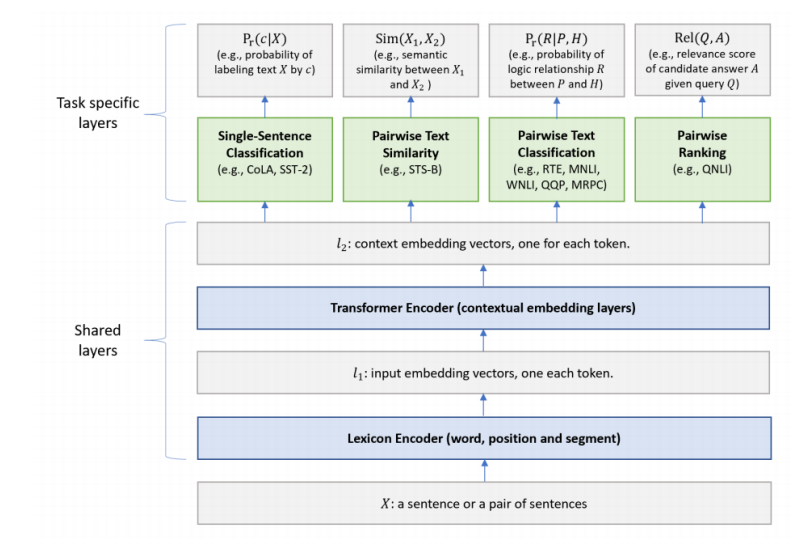
\includegraphics[width=\textwidth]{images/MTDNN1_.png}
 }
 \caption{Схема модели MT-DNN}\label{fig:MTDNN1}
\end{figure}

В задаче-специфичных слоях для решения задачи классификации,вычисление вероятности $P(x)$ (вектор вероятностей $P_{1}$,.... $P_{n}$ для принадлежности к классу $x_{1}$,... $x_{n}$) для векторного представления X токена [CLS] производится по формуле:

\begin{equation}
\color{black} P(x) = softmax(W^{T}X +B) \label{mtl:0}
\end{equation}

где $W^{T}$ матрица с тренируемыми коэффициентами размерности $H*n$, $H$ размерность скрытых состояний и $n$ число классов, B тренируемый вектор размерности $n$
В качестве функции потерь для данной задачи используется кросс-энтропия. 

Для решения задачи определения семантической близости (такой, как STS-B) используется похожая формула:

\begin{equation}
\color{black} S(x)=W^{T}X +B \label{mtl:1}
\end{equation}

где $W^{T}$ матрица тренируемых весовых коэффициентов размерности $H*1$, $H$ размерность скрытых состояний и 1 число классов, $B$ тренируемый весовой коэффициент размерности 1. 
Близость $S(x)$ может принимать значения от $-\inf$ до $\inf$. В качестве функции потерь используется среднеквадратичное отклонение.

Для задач классификации пары последовательностей в архитектуре MT-DNN используется стохастическая сеть ответов (stochastic answer network, SAN) \cite{liu_2018}. Данная нейросетевая архитектура, основанная на рекуррентных слоях Gated Recurrent Unit(GRU)\cite{cho_2014}, принимает на вход векторные представления пары последовательностей. На каждом шаге архитектура предсказывает возможные распределения вероятности между классами, что влияет на обновление весов модели. Финальные предсказанные вероятности получаются усреднением предсказанных вероятностей. 

Задача pairwise ranking (ранжирования пары последовательностей) решается аналогично предыдущим задачам, с соответствующими линейными трансформациями на входе и выходе.
Аналогичным же образом, с использованием линейных слоев, нейросетевая архитектура MT-DNN может быть адаптирована к решению задач распознавания именованных сущностей, что и было реализовано автором данной диссертационной работы в библиотеке DeepPavlov.

Как и оригинальный BERT, MT-DNN использует метод стохастического градиентного спуска для оптимизации функции потерь, подробнее описанный в \cite{bousquet_2004}. На каждом этапе модель формирует батч $B_{i}$ для решения целевой задачи i, дообучая классификаторы и параметры BERT в соответствии со спецификой задачи. 

Авторы оригинальной статьи производили дообучение модели BERT в соответствии со следующими параметрами: скорость обучения \num{5e-5}, оптимизатор Adamax \cite{kingma_2014}, размер батча 32, 5 эпох. 

Как показано в оригинальной статье, несмотря на отсутствие адаптации под конкретную задачу, модель MT-DNN превосходит BERT-LARGE на всех задачах, кроме CoLA. Как показано в \cite{na_2022}, отставание на задаче CoLA связано с особенностями данного набора данных. 

Также в оригинальной статье показано, что, после дообучения на каждую конкретную задачу модель MT-DNN показывает дополнительный прирост качества; на задачах с ограниченной обучающей выборкой (MRPC, RTE, SST-2) прирост может достигать 1-2.5\%. Это говорит о том, что модель MT-DNN может переиспользовать свои знания, полученные при обучении на задачах с более крупной обучающей выборкой, для решения задач с относительно маленькой выборкой.

Данные цифры показывают, что использование MT-DNN позволяет и экономить вычислительные ресурсы, и повышать при этом качество решения разных задач обработки естественного текста за счёт эффекта переноса знаний. 


\subsection{Модель PAL-BERT} 
Модель PAL-BERT, предложенная авторами статьи \cite{stickland_2019}, представляет собой вариант модульной нейросетевой многозадачной архитектуры. У нейросетевой модели в данном варианте есть задаче-специфичные слои с весами, отдельными для каждой конкретной задачичи общие слои. При этом часть задаче-специфичных слоев встраивается непосредственно «в тело» модели, основанной на архитектуре Трансформер. 

Слои, встраиваемые «в тело» такой модели, называются PALs - Projective Attention Layers (проективные слои внимания). Их действие описывается формулой

\begin{equation}
\color{black}PAL(h) = V_{d}*g(V_{e}*h) \label{mtl:2}
\end{equation}

где $V_{e}$ матрица кодировщика размерности $S$*$H$, H размерность вектора скрытого слоя $h$, $S$<$H$ (авторы статьи предложили $S$=204 для BERT-LARGE), $V_{d}$ матрица декодировщика размерности $H$*$S$ и где g - многоголовое внимание.

Матрицы $V_{d}$ и $V_{e}$ одни и те же для каждого слоя, но специфичные для каждой конкретной задачи. 
Эти слои добавляются авторами данной нейросетевой архитектуры в модель BERT следующим образом. Если выход каждого следующего слоя стандартной модели BERT $BERT_{i}$ зависит от выхода предыдущего слоя $BERT_{i-1}$ по формуле

\begin{equation}
\color{black}BERT_{i} =LayerNorm(BERT_{i-1})\label{mtl:3}
\end{equation},

то для модели PAL-BERT зависимость имеет такой вид:

\begin{equation}
\color{black}BERT_{i} =LayerNorm(BERT_{i-1} + PAL(BERT_{i-1})\label{mtl:4}
\end{equation}

\begin{figure}[ht]
 \centerfloat{
  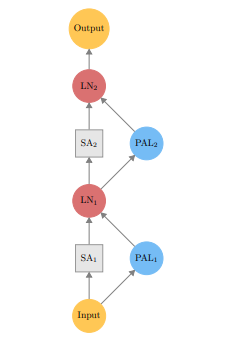
\includegraphics[width=0.6\textwidth]{images/PAL1_.png}
 }
 \caption{ Использование проективных слоев внимания(PAL1, PAL2) в модели PAL-BERT. LN означает LayerNorm, SA самовнимание.}\label{fig:PAL1}
\end{figure}


Использование архитектуры PAL-BERT увеличивает число параметров, необходимых для решения 8 задач GLUE,всего на 13 процентов. 
Авторы оригинальной статьи также применяли многозадачное обучение для модели PAL-BERT с использованием аннеалированного сэмплирования (annealed sampling). При использовании данного типа сэмплирования, вероятность выбора примера из i-того задания $P_{i}$ определяется следующим образом:

\begin{equation}
\color{black}P_{i} ~N^{(1-0.8*(e-1))/(E-1)}
\label{mtl:5}
\end{equation}
 
 где $e$ - номер эпохи, а $E$ - общее число эпох. 
 
Заметим, что полученные таким образом значения вероятностей нормируются на свою сумму. 

В связи с хорошими показателями и низким вычислительным бюджетом, модель PAL-BERT применялась как многозадачная модель на одном из этапов развития диалоговой системы DREAM, что подробнее описано в главе \ref{ch:mtldream}.

Однако отрицательным аспектом данной архитектуры является её негибкость и необходимость вручную подстраивать под каждую модификацию модели Transformer - а их на момент написания диссертации было разработано очень большое число, и регулярно появлялись новые модификации. В связи с необходимостью иметь возможность более «гибко» работать со всеми такими модификациями, было принято решение в дальнейшем использовать в диалоговой платформе {DREAM} неупрощенную версию трансформер-агностичной многозадачной нейросетевой модели, описанную в главе \ref{ch:tr-ag}.

Обзор самой диалоговой системы {DREAM} приведён в главе \ref{ch:dream}.

\subsection{Перенос знаний в многозадачных моделях}

В связи с тем, что в многозадачных нейросетевых архитектурах один и тот же её элемент в том или ином виде может использоваться для решения нескольких задач, возможна такая ситуация, когда знания, полученные при обучении модели решать одну из задач, помогают при решении и другой задачи. Т.е модель, которая обучалась решать задачу A и задачу B, может показать себя на задаче B лучше, чем если бы она обучалась решать только задачу A. Данный эффект называется переносом знаний, и его изучение является частью диссертационной работы.
